\begin{definition}[Causal pair]
  \label{def:causal_pair}
  Let $p_1:L_1{\remb} D_1 {\lemb} R_1$ and $p_2:L_2{\remb} D_2 {\lemb} R_2$ be two rules.

  A pair $P_1\overset{m_1,p_1}{\Rightarrow} M\overset{m_2,p_2}{\Rightarrow} P_2$ is a \emph{causal pair} if the cospan $R_1{\remb}M{\lemb}L_2$ is in the multisum of $R_1$ and $L_2$ and $p_1\redl{+}_s p_2$, where $s$ is the pullback of the cospan $R_1{\remb}M{\lemb}L_2$:
  \[
  \begin{tikzpicture} %[scale=0.8]
    \node (o) at (1,0) {\(O\)};
    \node (m) at (1,2) {\(M\)};
    \node (m1) at (-2,2) {\(P_1\)};
    \node (m2) at (4,2) {\(P_2\)};
    \node (r1) at (0,1) {\(R_1\)};
    \node (l1) at (-1,1) {\(L_1\)};
    \node (l2) at (2,1) {\(L_2\)};
    \node (r2) at (3,1) {\(R_2\)};
    \draw [left hook->] (o) -- (r1);
    \draw [left hook->] (o) -- (l2);
    \draw [left hook->] (r1) --  (m);
    \draw [left hook->] (l2) --  (m);
    \draw [left hook->] (l1) --  (m1);
    \draw [left hook->] (r2) --  (m2);
    \draw [>=latex, ->] (m1) -- node [above,midway] {$m_1,p_1$} (m);
    \draw [>=latex, ->] (m) -- node [above,midway] {$m_2,p_2$} (m2);
    \draw [>=latex, ->] (l2) -- (r2);
    \draw [>=latex, ->] (l1) -- (r1);
  \end{tikzpicture}
  \]
\end{definition}

\begin{lemma}
\label{lem:completeness_causal_pair}
  For each pair of sequential dependent transitions $G_1\overset{n_1,p_1}{\Rightarrow}G\overset{n_2,p_2}{\Rightarrow} G_2$ there exists a causal pair $M_1\overset{m_1,p_1}{\Rightarrow} M\overset{m_2,p_2}{\Rightarrow} M_2$ and a mono $h:M\emb G$ such that the following diagram commutes:
  \[
  \begin{tikzpicture} %[scale=0.8]
    \node (g) at (1,2.5) {\(G\)};
    \node (g1) at (-2,2.5) {\(G_1\)};
    \node (g2) at (4,2.5) {\(G_2\)};
    \node (m1) at (-2,1) {\(M_1\)};
    \node (m) at (1,1) {\(M\)};
    \node (m2) at (4,1) {\(M_2\)};
    \node (r1) at (0,-0.5) {\(R_1\)};
    \node (l1) at (-2,-0.5) {\(L_1\)};
    \node (l2) at (2,-0.5) {\(L_2\)};
    \node (r2) at (4,-0.5) {\(R_2\)};
    \draw [left hook->] (m) -- node [left,midway] {$h$} (g);
    \draw [left hook->] (m1) -- node [left,midway] {$h_1$} (g1);
    \draw [left hook->] (m2) --  (g2);
    \draw [>=latex, ->] (g1) -- node [above,midway] {$n_1,p_1$} (g);
    \draw [>=latex, ->] (g) -- node [above,midway] {$n_2,p_2$} (g2);
    \draw [>=latex, ->] (m) -- node [above,midway] {$m_2,p_2$} (m2);
    \draw [>=latex, ->] (m1) -- node [above,midway] {$m_1,p_1$}(m);
    \draw [left hook->] (r1) --  (m);
    \draw [left hook->] (l2) --  (m);
    \draw [left hook->] (l1) --  (m1);
    \draw [left hook->] (r2) --  (m2);
    \draw [>=latex, ->] (l2) -- (r2);
    \draw [>=latex, ->] (l1) -- (r1);
  \end{tikzpicture}
  \]
that is $n_1 = h_1\circ m_1$ and $n_2 = h\circ m_2$.

Moreover, for a causal pair $M_1\overset{m_1,p_1}{\Rightarrow} M\overset{m_2,p_2}{\Rightarrow} M_2$ and a mono $h:M\emb G$ such that the diagram above commutes, we have that the transitions $G_1\overset{n_1,p_1}{\Rightarrow}G\overset{n_2,p_2}{\Rightarrow} G_2$ are sequential dependent.
\end{lemma}
\begin{proof}
  First note that for any injective morphism in the diagram we can define a bijection between the domain and the image of the morphism in the codomain. For example, in the diagram above we have $m_2:L_2\to M$ an injective morphism; for any $x\in \text{image}(m_2)(L_2)$ the morphism $m_2^{-1}(x)$ is well defined.
  Secondly, we can always construct the pullback of the cospan $R_1\lemb G\remb L_2$ denoted $R_1\remb O \lemb L_2$ and the pullback of $K_1\lemb R_1\remb O$. We proceed by showing that in the diagram below
    \[
    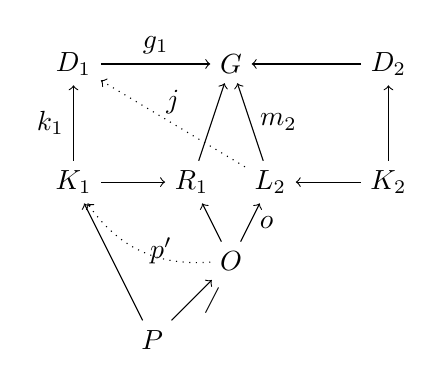
\begin{tikzpicture} %[scale=0.8]
    \node (r1) at (1.5,0) {\(R_1\)};
    \node (m1) at (2,1.5) {\(G\)};
    \node (l2) at (2.5,0) {\(L_2\)};
    \node (d1) at (0,1.5) {\(D_1\)};
    \node (k1) at (0,0) {\(K_1\)};
    \node (d2) at (4,1.5) {\(D_2\)};
    \node (k2) at (4,0) {\(K_2\)};
    \node (o) at (2,-1) {\(O\)};
    \node (p) at (1,-2) {\(P\)};
    \draw [->] (k1) -- (r1);
    \draw [->] (k2) -- (l2);
    \draw [->] (k1) -- node [left,midway] {\(k_1\)} (d1);
    \draw [->] (k2) -- (d2);
    \draw [->] (d1) -- node [above,midway] {\(g_1\)} (m1);
    \draw [->] (d2) -- (m1);
    \draw [->] (l2) -- node [right,midway] {\(m_2\)} (m1);
    \draw [->] (r1) -- (m1);
    \draw [dotted,->] (l2) -- node [above,midway] {\(j\)} (d1);
    \draw [->] (p) -- (k1);
    \draw [->] (p) -- node [right,midway] {$\not\iso$} (o);
    \draw [->] (o) -- (r1);
    \draw [->] (o) -- node [right,midway] {$o$} (l2);
    \draw [dotted,->] (o) to [bend left] node [right,midway] {$p'$} (k1);
    \end{tikzpicture}
    \]
    if the injective morphism $P\emb O$ is an iso then we can construct an morphism $j:L_2\to D_1$ that makes the diagram commute. We will have then a contradiction from which we can infer that indeed $P\emb O$ is not an iso. The construction of the causal pair $P_1\overset{m_1,p_1}{\Rightarrow} M\overset{m_2',p_2}{\Rightarrow} P_2$ follows straightforward from it.

    Suppose that $P\emb O$ is an iso. Let us show how we can recover from that a morphism $j:L_2\to D_1$.
    Let us denote $p:P\emb O$ the isomorphism between $P$ and $O$. Furthemore, we denote $p':O\to K_1$ the composition of $p$ and $P\to K_1$.
    Let $o(O) =L_2'\subseteq L_2$ be the image of $o:O\to L_2$. For any $x$ (node or edge) in $L_2'$, define $j(x) = k_1(p'(o^{-1}(x)))$. Consider now $x$ an edge or node in $L_2$ such that $x\notin L_2'$. We have that $m_2(x)\in G$ and moreover $m_2(x)\notin\text{image}(n_1)(R_1)$. The latter follows from $R_1 \remb O\lemb L_2$ being the pullback of $R_1\lemb G\remb L_2$. However $D_1\lemb G\remb R_1$ is the pushout of $D_1\remb K_1\lemb R_1$, hence $m_2(x)\in\text{image}(g_1)(D_1)$. $g_1$ is an injective morphism and therefore $g_1^{-1}(m_2)(x)$ is well defined. Then $j(x) = g_1^{-1}(m_2)(x)$. To summarise, $j$ is defined as follows
    \begin{align*}
      j(x) =& k_1(p'(o^{-1}(x))) &\text{for }x\in\text{image}(o)\subseteq L_2\\
      & g_1^{-1}(m_2(x))&\text{for }x\in L_2\setminus\text{image}(o).
    \end{align*}
and it is an injective morphism by construction. To show it commutes for the case when $x\in\text{image}(o)\subseteq L_2$ we use the fact that the graphs $O$ and $P$ are obtained by pullbacks.

In order to show the second part of the lemma, we will show that if there exists $j:L_2\to D_1$ then there exists a morphism $O\to P$ that makes the diagram commute. For any $x$ (node or edge) in $O$ we have that there exists $x_2\in\nodes_{L_2}$ such that $o(x_2)=x$ and similarly for $x_2\in\nodes_{L_2}$. As $O$ is the pullback, we have $m_2(x)\in G$ and moreover, $m_2(x_2)=g_1(j(x_2))$. Similarly, $n_1(x_1)=g_1(j(x_2))$. From the fact that the span $D_1\remb G\lemb R_1$ we have that there exists $x_k\in \nodes_{K_1}$ such that $k_1(x_k) = g_1(j(x_2))$ and $r_1(x_k)=x_1$. Then, as $P\to K_1$ is injective, we have that there exists $x_P\in\nodes_P$ such that $p(x)=x_p$ makes the diagram commute.
\end{proof}

\begin{definition}[Inhibiting pair]
  Let $p_1:L_1{\remb} D_1 {\lemb} R_1$ and $p_2:L_2{\remb} D_2 {\lemb} R_2$ be two rules.

  A pair $P_1\overset{m_1,p_1}{\Leftarrow} M\overset{m_2,p_2}{\Rightarrow} P_2$ is an \emph{inhibiting pair} if the cospan $L_1{\remb}M{\lemb}L_2$ is in the multisum of $L_1$ and $L_2$ and $p_1\redl{-}_s p_2$, where $s$ is the pullback of the cospan $L_1{\remb}M{\lemb}L_2$:
  \[
  \begin{tikzpicture} %[scale=0.8]
    \node (o) at (1,0) {\(O\)};
    \node (m) at (1,2) {\(M\)};
    \node (m1) at (-2,2) {\(P_1\)};
    \node (m2) at (4,2) {\(P_2\)};
    \node (l1) at (0,1) {\(L_1\)};
    \node (r1) at (-1,1) {\(R_1\)};
    \node (l2) at (2,1) {\(L_2\)};
    \node (r2) at (3,1) {\(R_2\)};
    \draw [left hook->] (o) -- (l1);
    \draw [left hook->] (o) -- (l2);
    \draw [left hook->] (l1) --  (m);
    \draw [left hook->] (l2) --  (m);
    \draw [left hook->] (r1) --  (m1);
    \draw [left hook->] (r2) --  (m2);
    \draw [>=latex, ->] (m) -- node [above,midway] {$m_1,p_1$} (m1);
    \draw [>=latex, ->] (m) -- node [above,midway] {$m_2,p_2$} (m2);
    \draw [>=latex, ->] (l2) -- (r2);
    \draw [>=latex, ->] (l1) -- (r1);
  \end{tikzpicture}
  \]
\end{definition}

\begin{lemma}
\label{lem:completeness_inhib_pair}
  For each pair of transitions $G_1\overset{n_1,p_1}{\Leftarrow}G\overset{n_2,p_2}{\Rightarrow} G_2$, where $G\overset{n_1,p_1}{\Rightarrow}G_1$ inhibits $G\overset{n_2,p_2}{\Rightarrow} G_2$ there exists an inhibiting pair $M_1\overset{m_1,p_1}{\Leftarrow} M\overset{m_2,p_2}{\Rightarrow} M_2$ and a mono $h:M\emb G$ such that the following diagram commutes:
  \[
  \begin{tikzpicture} %[scale=0.8]
    \node (g) at (1,2.5) {\(G\)};
    \node (g1) at (-2,2.5) {\(G_1\)};
    \node (g2) at (4,2.5) {\(G_2\)};
    \node (m1) at (-2,1) {\(M_1\)};
    \node (m) at (1,1) {\(M\)};
    \node (m2) at (4,1) {\(M_2\)};
    \node (l1) at (0,-0.5) {\(R_1\)};
    \node (r1) at (-2,-0.5) {\(L_1\)};
    \node (l2) at (2,-0.5) {\(L_2\)};
    \node (r2) at (4,-0.5) {\(R_2\)};
    \draw [left hook->] (m) -- node [left,midway] {$h$} (g);
    \draw [left hook->] (m1) -- node [left,midway] {$h_1$} (g1);
    \draw [left hook->] (m2) --  (g2);
    \draw [>=latex, ->] (g) -- node [above,midway] {$n_1,p_1$} (g1);
    \draw [>=latex, ->] (g) -- node [above,midway] {$n_2,p_2$} (g2);
    \draw [>=latex, ->] (m) -- node [above,midway] {$m_2,p_2$} (m2);
    \draw [>=latex, ->] (m) -- node [above,midway] {$m_1,p_1$} (m1);
    \draw [left hook->] (l1) --  (m);
    \draw [left hook->] (l2) --  (m);
    \draw [left hook->] (r1) --  (m1);
    \draw [left hook->] (r2) --  (m2);
    \draw [>=latex, ->] (l2) -- (r2);
    \draw [>=latex, ->] (l1) -- (r1);
  \end{tikzpicture}
  \]
that is $n_1 = h\circ m_1$ and $n_2 = h\circ m_2$.

Moreover, for any inhibiting pair $M_1\overset{m_1,p_1}{\Leftarrow} M\overset{m_2,p_2}{\Rightarrow} M_2$ and a mono $h:M\emb G$ such that the diagram above commutes, we have that the transition $G\overset{n_1,p_1}{\Rightarrow}G_1$ inhibits transition $G\overset{n_2,p_2}{\Rightarrow} G_2$.
\end{lemma}
The proof is similar to the one of \autoref{lem:completeness_causal_pair}.

\begin{remark}
  \autoref{lem:completeness_inhib_pair} is a weaker version of the completness result on critical pairs \cite{AlgebraicGR}.
\end{remark}
